\chapter{Implementação}

Após a definição das funcionalidades a instalar e da arquitectura de suporte, inicia-se o processo de desenvolvimento do comutador. Para isso procede-se a uma descrição em Verilog do design escolhido. Verilog é uma linguagem usada para descrever um bloco de \textit{hardware} no requerido fluxo de dados entre os vários registos presentes no mesmo. A esse tipo de descrição denomina-se \textit{Register Transfer Logic} (RTL). No design global do comutador foram incluídos dois modelos de RTL muito versáteis e comuns. São eles:

\begin{itemize}
  \item \textit{Finite State Machines} (FSM) -\quad Máquinas de estados são modelos abstratos de computação que dividem o funcionamento de um módulo em diferentes operações consoante o estado em que se encontram. As máquinas de estados definem não só os vários estados como as transições entre os mesmos, que podem depender do estado atual, dos vários sinais que são dados à máquina de estados por outros módulos, ou de ambos. São bastante utilizadas devido à simplicidade de descrição e aos baixos recursos requeridos na sua implementação.
   \item \textit{First-In-First-Out} (FIFO) -\quad FIFOs consistem num bloco de memória na qual os dados são lidos na mesma ordem da sua escrita. Normalmente são implementadas com recurso a dois ponteiros. Um ponteiro com a posição do endereço de memória onde será feita a escrita seguinte, e um ponteiro com a posição de memória onde deve ser feita a seguinte leitura. No momento de uma escrita ou leitura os dois ponteiros são incrementados para garantir a coordenação referida da ordem da escrita e leitura na memória. 
   \iffalse
    \item \textit{Dual-Port-RAM} (DPRAM) -\quad Memória RAM que, contrariamente às convencionais, permitem a escrita e leitura simultânea na mesma. No dispositivo desenvolvido é o caso das filas previamente descritas.
    \fi
\end{itemize}

\section{Interfaces}

Para proceder à troca de informação entre nós de uma rede de \textit{Ethernet} e os canais de comunicação, é necessário que se use uma interface reconhecida por ambos os elementos. Devido à existência das várias iterações da \textit{Ethernet} disponíveis hoje em dia definiram-se várias interfaces diferentes, usualmente indicadas para canais de um débito pré-especificado. O comutador desenvolvido nesta dissertação deverá ser incluído numa rede a operar com débitos de canal de 1000 Mbit/s. Para esses, a interface usada é, tipicamente, a \textit{Gigabit media-independente interface} (GMII). Nesta, a recepção e transmissão ocorre segundo uma frequência de 125 Mhz, onde são recebidos pelo nó 8 bits no flanco ascende do relógio associado à recepção, e transmitidos 8 bits no flanco ascendente do relógio associado à transmissão.
Nas tabelas 5.1 e 5.2 estão identificados e descritos, respetivamente, os sinais de recepção e transmissão da interface GMII.\par Como se pode observar na tabela 5.2, a interface GMII inclui dois relógios associados à transmissão. Um deles, o GTXCLK é usado quando se pretende transmitir dados com o débitos de 1000 Mbit/s, ao passo que o TXCLK é usado quando o débito pretendido é de 10 Mbit/s ou 100 Mbit/s. No comutador desenvolvido, havendo apenas ao momento a indicação do requerimento de suportar o débito de 1000 Mbit/s, somente se gera o relógio GTXCLK.


\begin{table}[h]
\begin{center}
\begin{tabular}{|l|l|}

    \hline
    Sinal &  Descrição  \\
    \hline
    RXCLK &  Pulso de relógio recebido  \\
    \hline
    RXD[7:0] & Dados recebidos \\
    \hline
    RXDV & Indica que os dados recebidos são válidos \\
    \hline
    RXER & Indica que os dados recebidos contêm erros \\
    \hline
    
\end{tabular}
\end{center}
\caption{Sinais de recepção da interface GMII}\label{Sinais de recepção do GMII}
\end{table} 

\begin{table}[h]
\begin{center}
\begin{tabular}{|l|l|}

    \hline
    Sinal &  Descrição  \\
    \hline
    GTXCLK &  Pulso de relógio de 1000 Mbit/s transmitido  \\
    \hline
    TXCLK &  Pulso de relógio de 10 ou 100 Mbit/s transmitido  \\
    \hline
    TXD[7:0] & Dados transmitidos \\
    \hline
    TXEN & Indica que os dados transmitidos são válidos \\
    \hline
    RXER & Indica que os dados transmitidos contêm erros \\
    \hline
    
\end{tabular}
\end{center}
\caption{Sinais de transmissão da interface GMII}\label{Sinais de transmissão do GMII}
\end{table}


\section{Modelo comportamental}

Nas secções seguintes será explicado detalhadamente de um posto de vista funcional o esquema interno do comutador desenvolvido com os seus vários módulos, o processamento interno de cada um, e os vários bits de informação que são trocados entre si. \par
O processo que decorre entre o início da recepção do preâmbulo de uma trama e a transmissão do término do FCS da mesma num porto diferente pode ser dividida, do ponto de vista dos módulos envolvidos, em 3 fases. Uma primeira fase na qual é procedida à recepção da trama, a criação de meta-dados da mesma fundamentais nas fases seguintes, e ao registo da trama e dos respetivos meta-dados nos vários blocos de memória presentes no comutador. Numa segunda fase, os módulos centrais do comutador, tais como a \textit{Switch Fabric}, procedem à lógica necessária para encaminhar as tramas dos blocos de memória onde se encontram para os portos de destino. Numa terceira fase é procedida a manipulações finais à trama que possam ser necessárias.   


\subsection{Recepção de uma trama}

Na figura 6.1 podem ser observados os vários módulos que participam no processo de recepção de uma trama num porto. Os módulos PTP \textit{Common Core} e \textit{Forward Logic} representados na imagem consistem em módulos centrais do comutador que comunicam com módulos presentes na fase de recepção de uma trama em todos os portos. Contrariamente, os restantes módulos observados são contidos no processo de recepção de um único porto, de forma que se replicam por todos os portos presentes no comutador. Alguns dos módulos possuem alguma complexidade, podendo conter submódulos. O funcionamento detalhado de cada um e alguns esquemas internos serão dados de seguida.  

\begin{figure}[H]
  \centering
  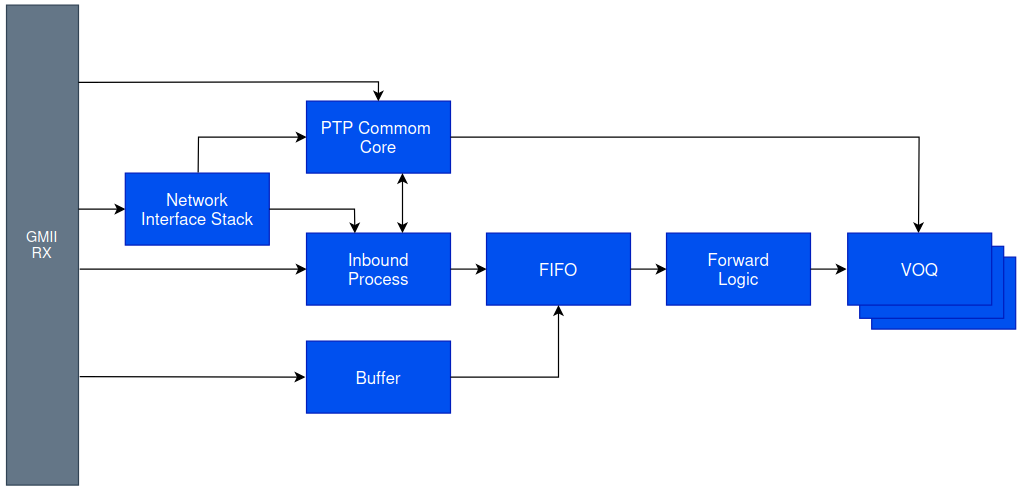
\includegraphics[width=1\textwidth]{FrameInbound.png}
  \caption[Processo de recepção de uma trama]{Processo de recepção de uma trama}
  \label{fig:airbus1}
\end{figure} 


\subsubsection{\textit{Inbound Process}}

O módulo \textit{Inbound Process} é o responsável por recolher um conjunto de meta-dados referentes ás tramas recebidas e por validar as mesmas para reencaminhamento. Para gerenciar a atividade do mesmo, este inclui uma máquina de estados. A máquina de estados é inicializada num estado de espera que remete a lógica de processamento de tramas do módulo para inatividade. Aquando da ativação do sinal RXDV avança-se sucessivamente para dois estados indicadores da recepção dos endereços MAC de destino e de origem da trama. Esses endereços são enviados para o módulo \textit{Forward Logic} onde serão usados no preenchimento e recolha de dados da tabela de endereços. Seguidamente, é identificado o \textit{EtherType} da trama. O valor do mesmo só é relevante se o mesmo for o \textit{EtherType} do PTP, o que é sinalizado ao módulo PTP \textit{Common Core}. Ainda que em certas normas como a IEEE 802.3 o campo que vem em seguimento ao campo do endereço MAC de origem possa comunicar o cumprimento do campo de dados da trama, o comutador recorre ao sinal \textit{RXDV} para delimitar a mesma. O último estado é aquele onde o módulo se encontra enquanto são recebidos o campo de dados e o FCS da trama, antes de voltar ao estado de espera. Há ainda um outro estado pelo qual o módulo pode passar caso seja identifica a presença da etiqueta de VLAN e de onde se recolhe a informação da prioridade da trama.   \par 
Se em qualquer momento durante o processamento da trama houver indicação de congestionamento da FIFO, indicação de congestionamento do \textit{Buffer}, indicação de que a trama é portadora de uma mensagem do PTP não passível de reencaminhamento, ou identificação de um erro, a trama não é aprovada para reencaminhamento e a decisão é comunicada ao \textit{Buffer}. Os erros possíveis de serem identificados pelo \textit{Inbound Process} são:

\begin{enumerate}
\item Erro no preâmbulo - \quad Erro identificado quando o preâmbulo e SFD não têm os valores esperados. 
\item Erro indicado pelo PHY - \quad Erro identificado quando o sinal RXER do respetivo porto se encontra com o valor lógico 1 aquando da recepção de um octeto da trama.
\item Erro no tamanho da trama -\quad Erro que ocorre quando o tamanho da trama é inferior ou superior aos limites definidos para as tramas do tipo \textit{Ethernet} II. Por forma a identificar este tipo de erro, o módulo inicia uma contagem aquando do início da recepção do campo de dados. Se suceder que a contagem ultrapasse o valor 1504 sem haver alteração do sinal RXDV, assume-se que a trama excedeu os 1500 octetos de dados permitidos somados aos 4 octetos do FCS. Da mesma forma, uma trama é interpretada como sendo demasiado pequena quando o valor do RXDV se torna 0 antes de a contagem chegar a 54, representativo dos 50 octetos do campo de dados mínimo somados aos 4 octetos de FCS. Futuramente, se, como é expectável, o comutador vier a ser incluído numa rede executante dos protocolos HSR ou PRP, os referidos valores dos limiares aceitáveis para o tamanho deverão ser ajustados para acomodar campos específicos dos referidos protocolos.  
\item Erro no FCS -\quad Aquando da mudança do sinal RXDV para 0, caso não tenha sido detetado um dos erros previamente descritos, pode ainda ser identificado um erro se o FCS que vem no fim da trama não coincidir com o FCS que é calculado no módulo. Um módulo capaz de calcular CRCs é incluído em cada módulo \textit{Frame Process} do comutador para esse efeito. 
\end{enumerate}

\subsubsection{\textit{Buffer}}

Blocos de memória na fase de recepção de tramas de um porto, onde é guardada a informação das referidas tramas, desde o preâmbulo até ao FCS. A estratégia escolhida passou por guardar as tramas num conjunto de segmentos de tamanho igual e pré-definido. Os segmentos precisam de ter uma dimensão suficiente para registar toda a informação referida anteriormente. Por exemplo, para uma situação em que o campo de dados tem o tamanho máximo de 1500 octetos, somando 22 octetos dos restantes campos, se se assumir 4 segmentos por trama, cada segmento deve ter capacidade para registar o mínimo de 593 octetos. Um exemplo de como as tramas podem ser guardadas num \textit{Buffer} pode ser observado na figura 6.2. Neste, podem ser identificadas duas tramas, a trama A e a trama B. A trama A está guarda nos segmentos com índice 1, 7 e 8, enquanto que a trama B está guardada nos segmentos com os índices 2, 3, e 6. Os restantes segmentos do \textit{Buffer} podem conter partes de tramas já recebidas ou encontrarem-se livres.


\begin{figure}[H]
  \centering
  \includegraphics[width=0.2 \textwidth]{Segments2.png}
  \caption[Buffer descontíguo]{Buffer descontíguo}
  \label{fig:airbus1}
\end{figure} 



 
O registo de uma trama no \textit{Buffer} no segmento disponível de índice mínimo inicia-se assim que o sinal TXDV é recebido com o valor lógico 1, marcando o segmento como indisponível numa tabela para isso criada. Após o preenchimento da totalidade do segmento, a escrita é transferida imediatamente para o segmento disponível seguinte, e assim sucessivamente, até que o sinal TXDV volte para o valor lógico 0. No final, se for recebida a informação por parte do módulo \textit{Inbound Process} que a trama não foi aprovada para reencaminhamento, os segmentos são novamente marcados como livres na lista sem haver necessidade de remover o conteúdo do \textit{Buffer}. A quantidade de leituras que deve ser feitas de cada segmento será dependente de a trama ser enviada em modo \textit{unicast} ou \textit{multicast}, sendo essa informação disponibilizada posteriormente pelo módulo que gere as VOQ. 

\subsubsection{PTP \textit{Common Core}}

O módulo PTP \textit{Common Core} é onde são analisadas as mensagens do protocolo \textit{PTP} e geradas as respostas em concordância com o protocolo. Na figura 5.3 está ilustrada a estrutura simplificada do módulo. Por forma a possibilitar a recepção de tramas portadoras de mensagens do PTP em todos os portos do comutador em simultâneo existe uma estrutura destas dedicada a cada porto. 


\begin{figure}[H]
  \centering
  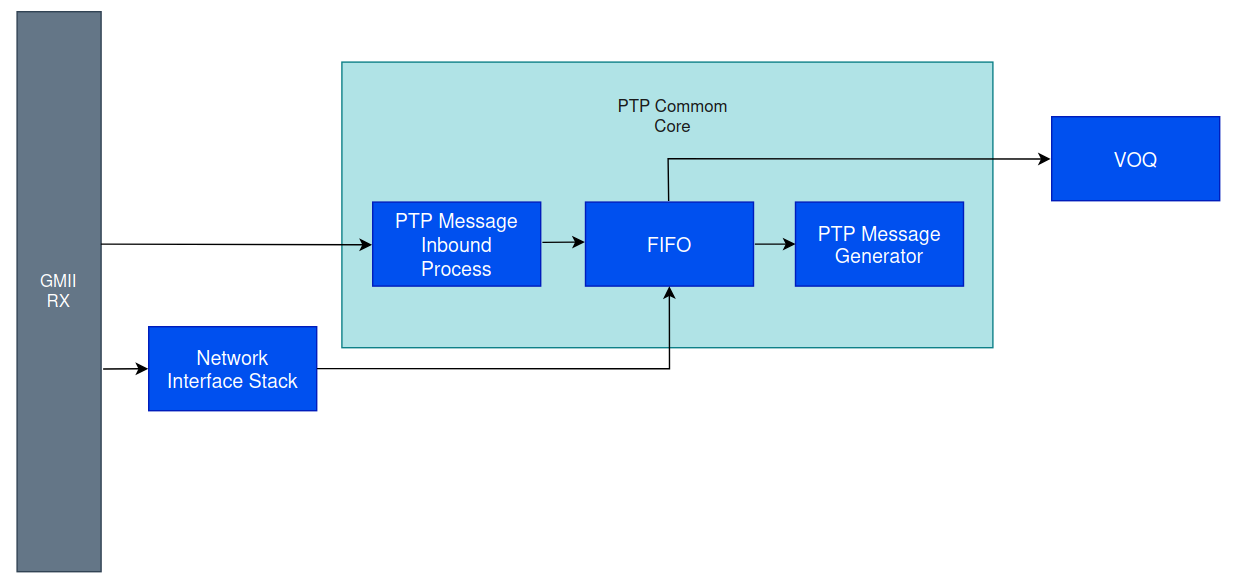
\includegraphics[width=1 \textwidth]{CommomCore.png}
  \caption[PTP Commom Core]{PTP Commom Core}
  \label{fig:airbus1}
\end{figure} 

O módulo PTP \textit{Message Inbound Processo} é onde são analisadas as mensagens do PTP recebidas e tomadas as decisões sobre como proceder. As quatro decisões possíveis, cujas circunstâncias causadoras foram explicadas no subcapítulo 2.4.1 são as seguintes:

\begin{enumerate}
    \item -\quad Permitir o reencaminhamento da trama sem requeres a alteração do \textit{correctionField}.
    \item -\quad Permitir o reencaminhamento da trama requerendo a alteração do \textit{correctionField}.
    \item -\quad Unicamente descartar a trama.
    \item -\quad Descartar a trama e iniciar o processo de resposta com uma trama portadora de uma mensagem \textit{PDelay\_Resp}.
\end{enumerate}

Quando é tomada a decisão de gerar uma mensagem \textit{PDelay\_Resp}, os campos \textit{sequenceId}, \textit{sourcePortIdentity}, \textit{correctionField}, e instante de recepção da mensagem \textit{PDelayReq} são capturados e colocados na FIFO presente no PTP \textit{Common Core}, onde aguardam até poderem ser inseridas na VOQ correspondente. Também na mesma FIFO são inseridas as indicações do requisito de transmissão das mensagens \textit{PDelay\_Req} nos momentos oportunos. 
 

\subsubsection{FIFO}
FIFOs onde são guardados os meta-dados referentes a uma trama. Os meta-dados consistem no tamanho da trama, o endereço MAC de destino e origem, a prioridade da mesma, um bit identificador de uma mensagem PTP da classe evento, o instante de recepção pelo comutador e os índices dos segmentos do \textit{Buffer} onde é guardada a trama. Um bit sinalizador do estado de FIFO vazia é fornecido ao módulo \textit{Frame Process} enquanto que outro sinalizador de FIFO cheia é fornecido ao módulo MAC \textit{Table Controller}. 


\subsubsection{\textit{Forward Logic}}

O módulo \textit{Forward Logic} é o responsável por proceder à gestão da tabela de endereços com recurso ao algoritmo explicado no capítulo 4. O módulo é único no comutador e recebe como sinais de entrada os bits indicadores de se as FIFO's previamente mencionadas se encontram ou não vazias. O módulo tem um estado de espera predefinido durante o qual aguarda que alguma fila deixe de estar vazia. Quando o bit de entrada de uma das vilas indica que esta não se encontra vazia, o módulo MAC \textit{Forward Logic} requer a leitura do elemento no topo da fila onde se encontram, entre outros dados, o endereço MAC de destino e origem da trama. Seguidamente, o módulo procede ao cálculo do CRC dos endereços MAC de destino e origem da trama que é usado como função de dispersão. Após o cálculo dos CRC's, é executada a procura dos endereços e possível atualização da tabela como explicado no capítulo 4. Para minimizar o tempo que uma trama se encontra no comutador, a procura do endereço de destino incluído na trama é efectuada antes da procura pelo endereço de origem. A conclusão do processo de procura do endereço de destino, juntamente com a informação do porto ou portos de destino da mesma, são imediatamente comunicados ao módulo responsável por atualizar as VOQs. 

\subsubsection{VOQ}

Filas de metadados referidas no capítulo 4. A quantidade de VOQs instaladas na fase de recepção de cada porto é dada pelo produto da quantidade de portos do comutador pela quantidade de prioridades de transmissão definidas. Os referidos metadados consistem nos índices dos vários segmentos do \textit{Buffer} onde se encontra guardada a trama, o instante de recepção da trama pelo porto, o tamanho da trama, e um código que indica se a trama contém uma mensagem do PTP.  A inserção é efectuada após a indicação do porto de destino da trama ou da transmissão em modo \textit{broadcast} por parte do módulo \textit{Forward Logic}. Quando a indicação é de proceder à transmissão para um único porto, os metadados são inseridos na VOQ correspondente ao porto destino e à prioridade da trama comunicada pelo módulo \textit{Inbound Process}. Alternativamente, quando a indicação é para reencaminhar a trama em modo \textit{broadcast}, os meta-dados são inseridos em todas as filas da respetiva prioridade, excluindo a fila que reencaminharia a trama de regresso ao porto por onde foi recebida.\par
 A inserção dos metadados referentes a tramas portadoras de mensagens \textit{PDelay\_Req} e \textit{PDelay\_Resp} ocorre quando solicitada pelo módulo PTP \textit{Common Core}, e é efectuada numa VOQ que represente o envio de uma trama de um porto para si mesmo. Para estas, os metadados consistem apenas no código respectivo Para reduzir o tempo que as tramas portadoras de mensagens do PTP permanecem no comutador, os seus metadados são sempre inseridos em filas de prioridade máxima.


\subsection{Reencaminhamento das tramas}

O processo de reencaminhamento das tramas é executado por dois módulos, \textit{Switch Fabric} e \textit{Switch Fabric Interface}. O módulo \textit{Switch Fabric} é exclusivamente responsável por receber os pedidos de transmissão de cada porto, selecionar os reencaminhamentos e providenciar os vários percursos que permitam a execução desses reencaminhamentos de tramas entre os portos. 
Por sua vez, o módulo \textit{Switch Fabric Interface} é responsável por proceder à comunicação entre os módulos da fase de recepção de tramas, os módulos que procedem às manipulações das tramas em fase de transmissão, e a \textit{Switch Fabric}. 
Seguidamente, segue uma descrição do funcionamento isolado de ambos.



\subsubsection{\textit{Switch Fabric}}

Na figura 5.4 é possível ser observada uma versão simples da estrutura interna do módulo \textit{Switch Fabric}.

\begin{figure}[H]
  \centering
  \includegraphics[width=0.3 \textwidth]{Fabric.png}
  \caption[\textit{Switch Fabric}]{\textit{Switch Fabric}}
  \label{fig:airbus1}
\end{figure} 

O seu submódulo principal é aquele denominado de iSLIP que executa o algoritmo homónimo descrito no capítulo 3. Por forma a maximizar sempre a correspondência entre portos a requerer o reencaminhamento de tramas, e os portos disponíveis para as receber, o módulo executa várias iterações do algoritmo até que não haja mais correspondências possíveis. \par Tal como muitos dos restantes módulos do comutador, este inclui uma máquina de estado para controlar a execução do algoritmo. Por defeito, a máquina de estados encontra-se num estado de espera, na qual o módulo iSLIP se encontra inativo. A transição para execução do algoritmo ocorre quando são transmitidos os pedidos de reencaminhamento de tramas por parte do módulo \textit{Switch Fabric Interface}. A execução do algoritmo decorre durante um único estado. Cada iteração decorre durante um ciclo de relógio desse estado, percorrendo os três estágios necessários: \textit{request}, \textit{grant} e \textit{accept}. No final da iteração, se for efectuada uma nova correspondência, o estado mantém-se, executando-se uma nova correspondência entre os portos não envolvidos nas correspondências já estabelecidas. Aquando da conclusão de uma iteração que não produza correspondências, a informação das correspondências estabelecidas é comunicada à \textit{Switch Fabric Interface}, e avança-se para um novo estado. Neste, decorre o envio do conteúdo das tramas dos portos de origem para os portos de destino através da matriz \textit{crosspoint} presente na \textit{Switch Fabric}. Esta consiste numa matriz de pontos de interseção que possuem dois conjuntos de entradas e saídas, e dois estados possíveis, representativos das duas formas possíveis de proceder a uma ligação bijetiva entre os referidos conjuntos. Uma representação da matriz pode ser observada na figura 5.5, juntamente com os respetivos pontos de interseção na figura 5.6.

\begin{figure}[H]
\centering
\begin{minipage}{.5\textwidth}
  \centering
  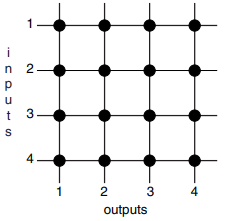
\includegraphics[width=.9\linewidth]{crossmatrix.png}
  \caption{Matriz \textit{crosspoint}}{(fonte: \cite{math})}
  \label{fig:test1}
\end{minipage}%
\begin{minipage}{.5\textwidth}
  \centering
  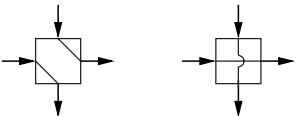
\includegraphics[width=.9\linewidth]{crosspoint.png}
  \caption{Ponto de interseção}{(fonte: \cite{math})}
  \label{fig:test2}
\end{minipage}
\end{figure}

A decisão sobre estados dos pontos de interseção que criam os caminhos entre os portos que possuem tramas a transmitir e os portos de destino correspondentes é efectuada pelo submódulo \textit{Matrix Control}. Para uma correta tomada de decisão a informação das correspondências é-lhe transmitida pelo módulo responsável por executar o iSLIP. 
Quando as tramas tiverem sido integralmente transmitidas, a conclusão do processo é comunicada pela \textit{Switch Fabric Interface}, regressando a \textit{Switch Fabric} a um estado de espera.  

\subsubsection{\textit{Switch Fabric Interface}}

O módulo \textit{Switch Fabric Interface} consiste num ponto de comunicação entre os módulos presentes na recepção e transmissão das tramas, e a \textit{Switch Fabric}, como pode ser observado na figura 5.7.

\begin{figure}[H]
  \centering
  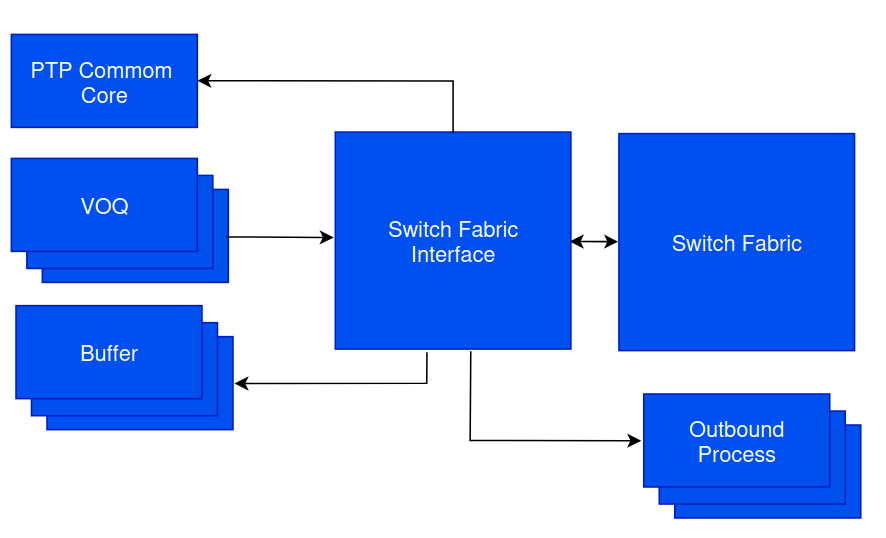
\includegraphics[width=1 \textwidth]{Interface_Fabric.png}
  \caption[\textit{Switch Fabric Interface}]{\textit{Switch Fabric Interface}}
  \label{fig:airbus1}
\end{figure} 


Esta é responsável por comunicar os pedidos de transmissão de tramas à \textit{Switch Fabric}, e, após providenciada a correspondência, requerer a leitura dos segmentos de memória dos \textit{Buffer}s onde estão guardadas as tramas. Ainda que haja troca de conteúdo das tramas entre a \textit{Switch Fabric} e outros módulos como o \textit{Buffer}, a responsabilidade da comunicação dos momentos adequados para a efectuar é da inteira responsabilidade da \textit{Switch Fabric Interface}.   \par
Para tirar o máximo de proveito das características da \textit{Switch Fabric} e do iSLIP, o momento em que é feito um novo pedido à \textit{Switch Fabric} situa-se imediatamente a seguir ao envio de todas as tramas por parte dos portos servidos previamente pela \textit{Switch Fabric}. Aí, para a criar o novo pedido de correspondências, a \textit{Switch Fabric Interface} apenas precisa de analisar o valor de um conjunto de sinais que indicam se as VOQs presentes no comutador estão, ou não, vazias.  


\subsection{Transmissão de uma trama}

Após a recepção na \textit{Switch Fabric Interface} da correspondência selecionada pela \textit{Switch Fabric} inicia-se o processo de envio das tramas para fora do comutador. Os módulos envolvidos na transmissão e as operações por si efectuadas variam consoante a trama seja gerada no comutador ou apenas reencaminhada. Seguidamente segue uma descrição das duas variantes do processo.

\subsubsection{Transmissão de tramas reencaminhadas}

Na figura 5.8 estão ilustrados os módulos que participam na transmissão de uma trama guardada num \textit{Buffer} do comutador após indicação do início do reencaminhamento por parte da \textit{Switch Fabric Interface}.

\begin{figure}[H]
  \centering
  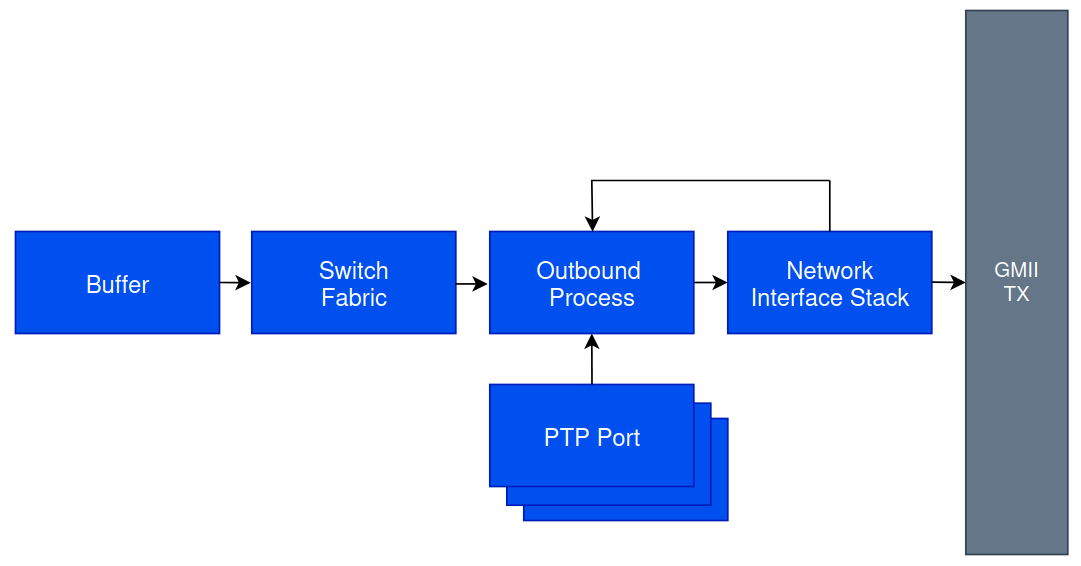
\includegraphics[width=1 \textwidth]{Outbound_Normal.png}
  \caption[Transmissão de tramas reencaminhadas]{Transmissão tramas reencaminhadas}
  \label{fig:airbus1}
\end{figure} 

Como explicado previamente, o conteúdo das tramas é guardada em segmentos dos \textit{Buffers} nos portos de recepção. Os ponteiros para as posições iniciais de cada segmentos são inseridos nas VOQs adequadas e recolhidos mais tarde pelo módulo \textit{Switch Fabric Interface} após a indicação por parte da \textit{Switch Fabric} de que pode começar a transmissão da referida trama. Assim que a \textit{Switch Fabric Interface} se encontre em posse dos ponteiros, esta indica aos \textit{Buffers} a leitura das tramas. \par 


Antes de sair do comutador, o fluxo de dados vindo dos \textit{Buffers} atravessa o módulo \textit{Outbound Process}. Este módulo, após receber a indicação do início da transmissão por parte da \textit{Switch Fabric Interface}, é responsável por fazer duas manipulações ao fluxo de dados recebido antes de o reencaminhar para a interface GMII. 

\begin{enumerate}
\item Alteração do \textit{correctionField} -\quad Para algumas mensagens do PTP já mencionadas anteriormente é necessário adicionar o tempo de residência e, em situações mais específicas, o \textit{meanLinkDelay} associado ao porto. O código identificador dessas mensagens é comunicado ao \textit{Outbound Process} pela \textit{Switch Fabric Interface}. Uma vez que, tanto as tramas de \textit{Ethernet} como as mensagens do PTP seguem um formato fixo, a posição do \textit{correctionField} na trama é constante para as tramas padronizadas da \textit{Ethernet}. Assim, para determinar o momento de manipulação do \textit{correctionField}, o módulo apenas precisa de iniciar uma contagem aquando do início da transmissão da trama que decorra até à posição previamente calculada do \textit{correctionField}. O instante de recepção da trama por um porto, de transmissão no porto adequado, e o \textit{meanLinkDelay}, são fornecidos ao módulo respetivamente pela \textit{Switch Fabric Interface}, \textit{Network Interface Stack} e PTP \textit{Port}.
\item Alteração do FCS -\quad Quando há alteração do \textit{correctionField} torna-se necessário calcular um novo FCS para a trama. Para isso, as tramas que são transmitidas por um porto são fornecidas a um módulo que calcula CRCs igual ao que se encontra presente no módulo \textit{Inbound Process}. No entanto, a responsabilidade de indicar o início e o fim da trama ao respetivo módulo e de inserir o código gerado na trama é da responsabilidade do \textit{Outbound Process}. A informação do tamanho da trama para isso necessária é-lhe fornecida pelo módulo \textit{Switch Fabric Interface}.
\end{enumerate}

\subsubsection{Transmissão de tramas \textit{PDelay\_Req} e \textit{PDelay\_Resp}}

Os módulos envolvidos na geração e consequente transmissão de uma trama portadora de uma mensagem \textit{PDelay\_Req} ou \textit{PDelay\_Resp} podem ser observados na figura 5.9.


\begin{figure}[H]
  \centering
  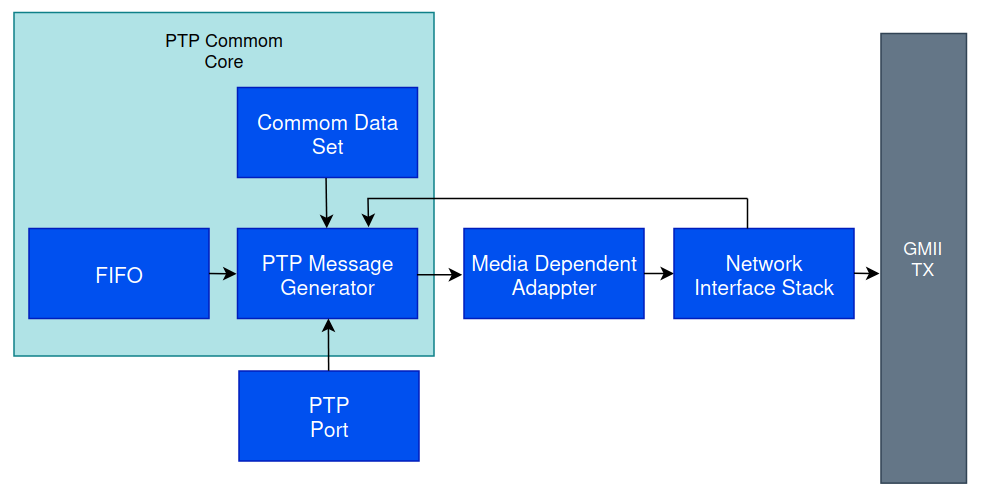
\includegraphics[width=1\textwidth]{PTP_Commom_Core.png}
  \caption[Transmissão de tramas \textit{PDelay\_Req} e \textit{PDelay\_Resp}]{Transmissão de tramas \textit{PDelay\_Req} e \textit{PDelay\_Resp}}
  \label{fig:airbus1}
\end{figure} 


Para facilitar a inclusão da capacidade de geração de tramas por iniciativa própria por parte do comutador, as tramas portadoras de mensagens \textit{PDelay\_Req} e \textit{PDelay\_Resp} requerem o acesso à \textit{Switch Fabric} em igualdade com as restantes tramas, ainda que não necessitem de reencaminhamento de um porto para outro. Desta forma, o início do envio destas tramas coincide com o início do envio de tramas reencaminhadas. Nesse instante, a \textit{Switch Fabric Interface}, com o conhecimento obtido através do código inserido na respetiva VOQ, informa o PTP \textit{Common Core} da autorização para a transmissão da respetiva trama portadora de uma mensagem \textit{PDelay\_Req} ou \textit{PDelay\_Resp}. A geração da trama começa, por indicação do PTP \textit{Common Core}, no módulo MD \textit{Adapter} presente no porto. Este é responsável por gerar todos os campos da trama à exceção do campo de dados com os seguintes conteúdos:


\begin{itemize}
  \item Preâmbulo -\quad 7 octetos com o valor 8xD5.
  \item SFD - \quad Um octeto com o valor 8x55.
  \item Endereço MAC de destino - \quad Como definido na norma, 01-80-C2-00-00-0E quando a trama contém uma mensagem utilizada no mecanismo P2P e 01-1B-19-00-00-00 para tramas que contenham uma das restantes mensagens.
  \item Endereço MAC de origem - \quad Endereço MAC do comutador que lhe é dado como parâmetro no código Verilog desenvolvido.
  \item \textit{EtherType} -\quad O \textit{EtherType} do PTP definido na norma, 16x88F7.
\end{itemize}


Após o preenchimento dos referidos campos, o MD \textit{Adapter} comunica ao PTP \textit{Common Core} o início da geração e transmissão do campo de dados.\par Para permitir a criação de mensagens relativas ao mecanismo P2P em simultâneo em todos os portos, o módulo PTP \textit{Common Core} possui um gerador dessas mensagens dedicado a cada porto. Esse gerador é responsável por preencher os vários campos do cabeçalho e corpo das mensagens com os vários valores das estruturas de dados presentes nos módulos PTP \textit{Port} e PTP \textit{Common Core}, e, no caso das mensagens \textit{PDelay\_Resp}, com recurso a alguns campos da mensagem \textit{PDelay\_Req} à qual se está a responder e do instante de transmissão da mensagem \textit{PDelay\_Resp}. Os dados provenientes da mensagem \textit{PDelay\_Req} são recolhidos da fila após a comunicação por parte da \textit{Switch Fabric Interface} da autorização para gerar a trama respetiva. O instante de transmissão da trama, necessário para preencher o \textit{correctionField} de uma mensagem do tipo \textit{PDelay\_Resp} é transmitido ao gerador pela \textit{Network Interface Stack} do respetivo porto.\par     
No fim da geração da mensagem do PTP o evento é comunicado ao \textit{MD Adapter}. Quando a mensagem a ser gerada é do tipo \textit{PDelay\_Resp}, este insere na trama o FCS calculado pelo módulo por isso responsável finalizando a criação da mesma.

\subsection{Cálculo do \textit{meanLinkDelay}}
O cálculo do \textit{meanLinkDelay} de um porto é da responsabilidade do respetivo PTP\textit{Port}. Nestes, cada um possui um contador que é incrementado todos os ciclos de relógio até decorrer 1 segundo que é o tempo de intervalo entre transmissões sucessivas de mensagens \textit{PDelay\_Req} definido na norma. Aí, o PTP \textit{port} requer o envio da mensagem ao PTP \textit{Commom Core} e fornece o \textit{sequenceId} respetivo ao mesmo. No momento em que a mensagem começa a ser gerada, o instante de transmissão da mesma, fornecido pelo \textit{Nerwork Interface Stack}, é registado pelo PTP \textit{Port}, assim como a sua associação ao \textit{sequenceId} da mensagem. O cálculo do \textit{meanLinkDelay} inicia-se no momento da recepção de uma mensagem \textit{PDelayResp} se o PTP \textit{Port} estiver a aguardar uma mensagem com o \textit{sequenceId} que vem na mesma e se o \textit{twoStepFlag} tiver o valor 0. Se o \textit{twoStepFlag} tiver o valor 1, o instante de recepção da mensagem, o seu \textit{correctionField} e o seu \textit{requestReceiptTimestamp} são registados em associação com o \textit{sequenceId} da mensagem. Aí, o cálculo acontece no momento da recepção da mensagem \textit{Pdelay\_Resp\_Follow\_Up} com o mesmo \textit{sequenceId}.\par
No instante em que o PTP \textit{Port} toma a decisão de atualizar o \textit{meanLinkDelay} as grandezas usadas são fornecidas a uma calculadora a isso dedicada. Dada a dimensão elevada dessas grandezas em quantidade de bits, para a calculadora ser sintetizável, as várias multiplicações e somas realizadas tiveram que ser subdivididas em operações com operandos de menor dimensão. 


\section{Opções de configuração}

Para tirar proveito da reconfigurabilidade das FPGA's, durante o desenvolvimento do comutador, o código Verilog do mesmo foi preferencialmente elaborado com recurso a parâmetros. Isso permite aumentar o conjunto de ambientes nos quais o comutador possa ser instalado, manipulando os parâmetros necessários. Os parâmetros existentes são os seguidamente descritos.

\begin{itemize}
  \item NUMBER\_PORTS  - \quad Define a quantidade de portos de Ethernet presentes no comutador. 
  \item SEGMENT\_SIZE  - \quad Define a quantidade de endereços de memória consecutivos num \textit{Buffer} que perfazem um segmento. 
  \item TOTAL\_SEGMENTS - \quad Define a quantidade de segmentos existentes no \textit{Buffer} associado a um porto.
  \item BIN\_SIZE - \quad Define o tamanho dos vários \textit{Buffers} circulares presentes na tabela de endereço.
  \item MAC\_TABLE\_SIZE - \quad Define a quantidade de \textit{Buffers} circulares presentes na tabela de endereços.
  \item VOQ\_FIFO\_SIZE -\quad Define a quantidade de elementos que podem ser armazenados em cada uma das várias VOQ's presentes no comutador. Precisa de ser um múltiplo de 2.
  \item PRIORITY\_QUEUE -\quad Define a quantidade de prioridades de diferentes com que as tramas podem ser diferenciadas pelo comutador. O valor deste parâmetro reflete-se na quantidade de VOQs que podem representar o envio de tramas entre cada par de portos.
  \item SLIP\_STAGES -\quad Define a quantidade de módulos consecutivos capazes de executar uma iteração do algoritmo iSLIP. Valores mais elevados neste parâmetro garantem uma execução mais rápida do iSLIP, pagando o custo de necessitar de mais recursos na implementação em FPGA.
  \item PTP - \quad Parâmetro que promove a instanciação de toda a lógica necessária para executar o protocolo PTP quando lhe é atribuido o valor 1. 
  \item COUNTERS - \quad Parâmetro que promove a instanciação de contadores de tramas úteis para calcular o desempenho do comutador e auxiliar em situações de depuração. Estes contadores permitem o registo da quantidade de tramas recebidas pelo comutador, a quantidade de tramas aprovadas para reencaminhamento, a quantidade de tramas rejeitadas por conterem erros, a quantidade de tramas descartadas por congestionamento de um \textit{Buffer}, a quantidade de tramas rejeitadas por congestionamento de uma VOQ, a quantidade de tramas transmitidas pelo comutador, e total de octetos contabilizados nas situações referidas. 
  \item ASYNC\_FIFO - \quad Quando com o valor 1, este parâmetro promove a instanciação de filas assíncronas, explicadas no capítulo seguinte.
\end{itemize}
  
Além dos referidos parâmetros, o comutador inclui ainda dois registos de configuração responsáveis por, separadamente, activar e desactivar o funcionamento como E2E \textit{Transparent clock} e P2P \textit{Transparent Clock}. 